\hspace{24pt}

Over the past few years, the field of neural machine translation (NMT) between Chinese and Japanese is still an unresolved problem. Recent studies in Chinese-Japanese NMT have used specific methods such as sub-character level features to improve the translation quality. This is due to the lack of parallel corpus and the difference between logogram (a character or symbol that represents a word) and alphabet (a set of letters used when writing in a language) writing systems. This research explores phonetic information as an additional feature for improving the quality of Chinese-Japanese NMT systems.

\section{Background} \label{sec:background}

NMT is a popular area of natural language processing (NLP), has been proposed by using an end-to-end model which transforms a source sentence into a latent space and decodes it directly into a target sentence \cite{sutskever2014sequence, cho2014learning}. The model is called the encoder-decoder model or sequence-to-sequence model, and they are widely used by large technology companies such as Google, Facebook, Microsoft, and DeepL.

\subsection{Progress of Neural Machine Translation} \label{sec:nmt}

The progress of NMT and NLP are inseparable. The development of models, tokenization methods, embeddings, and the solutions to less or no parallel data, all involved in the progress of NMT.

Recurrent neural networks (RNNs), attention mechanisms, and transformers have been proposed sequentially throughout the progress of encoder-decoder models. RNN that recursively passes states in its networks was first applied in the encoder-decoder model \cite{cho2014learning}. Attention-mechanism had addressed the problem of insufficient information in the latent space between encoder and decoder based on RNN \cite{bahdanau2014neural}. Transformers had replaced the RNN structure with full attention-mechanism (i.e., self-attention) to achieve better results and used widely in NMT tasks \cite{NIPS2017_3f5ee243}. 

Tokenization is one of the most important parts of any NLP task. It determines how a sentence will be tokenized, and it will generate different meanings to a sentence with different algorithms. Besides word-level and character-level tokenization, several subword-level tokenization algorithms had become the mainstream. For example: Byte-Pair Encoding (BPE) \cite{sennrich_neural_2016}, Unigram Language Model \cite{kudo-2018-subword}, WordPiece \cite{6289079}, and SentencePiece \cite{kudo-richardson-2018-sentencepiece}. This paper will utilize BPE, SentencePiece \cite{sennrich_neural_2016, kudo-richardson-2018-sentencepiece} and two word-level tokenizer (\textit{Jieba}\footnote{https://github.com/fxsjy/jieba} and \textit{Janome}\footnote{https://mocobeta.github.io/janome}) as tokenization methods.

The concept of embeddings, also known as distributed representations, was first proposed by \cite{hinton1986learning, bengio2003neural}, but was difficult to implement due to hardware limitations. With the development of parallel computing and GPU, many embedding implementations have been proposed, such as Word2Vec \cite{mikolov2013efficient}, GloVe \cite{pennington2014glove}, and fastText \cite{bojanowski2017enriching}. The contextualized word embedding is another concept that obtains context-dependent word embedding from the whole sentence, meaning that the same word with a different position can obtain different embedding through the model. The representative ones are ELMo \cite{peters-etal-2018-deep} and BERT \cite{devlin-etal-2019-bert}. This paper will select Word2Vec \cite{mikolov2013efficient} as the tool for creating word embeddings because of its simplicity, rapidity, and convenience of analysis.

Several fields have been studied to solve the problems like low-resources and noisy parallel data in NMT tasks. Back-translation \cite{sennrich-etal-2016-improving} is a data augmentation method that uses monolingual data of the target language to generate source data and offset the imbalance between encoder and decoder. Parallel corpus filtering was examined for a large number of NMT tasks \cite{koehn2018findings}, using pre-filtering rules and scoring functions to retain good sentence pairs can effectively reduce the corpus size and obtained better translation results. This paper will practice corpus filtering to retain quality training data and reduce corpus size to increase experimental efficiency.

\subsection{Chinese-Japanese Neural Machine Translation}

NMT system has gained a lot of improvement in translating between English and other languages by utilizing the techniques described in section \ref{sec:nmt}. However, the improvement in translating between Chinese and Japanese is limited. The main reasons are the inadequacy of the corpus and the differences in the writing systems of Chinese, Japanese, and Western languages.

Many studies have focused on improving the Chinese-Japanese (zh-ja) NMT system. In addition to using the methods \cite{imamura2018enhancement, chu2017empirical, zhang2020parallel} described in section \ref{sec:nmt}, many feature engineering techniques have been proposed to utilize the features in Chinese Characters (\textit{Hanzi}) and Japanese \textit{Kanji}. For example, a character-level zh-ja NMT system had been improved by using radicals as character feature information \cite{8300572}. Furthermore, the use of decomposed sub-character level information such as ideographs and strokes of Chinese characters, also improved the results \cite{zhang-komachi-2018-neural}.

\subsection{Phonetic Information} \label{sec:phonetic}

Phonetic information is another feature that had been applied to NMT systems. \cite{khan2019diversity} had suggested that a phonetic representation usually corresponds to semantically distinct characters or words. \cite{liu-etal-2019-robust} had pointed out that phonetic information can effectively resist the homophone noises generated by typographical mistakes in Chinese sentences. Both papers had improved the performance of the NMT system between Chinese and other Western languages.

This paper attempts to use \textit{Bopomofo} and \textit{Hiragana} as Chinese and Japanese phonetic information to improve the performance of the zh-ja NMT system. Bopomofo also named \textit{Zhuyin} (注音), is located in the Unicode block in the range U+3100–U+312F. It consists of 37 characters and 4 tone marks to transcribe all possible Chinese characters. Although it is the main component of Mandarin Chinese, it usually does not appear in Chinese sentences. That is, the machine loses some of the phonetic information when reading Chinese sentences. \begin{CJK}{UTF8}{song}
Hiragana (平仮名, ひらがな) is a component of Japanese, along with \textit{Katakana} and Kanji. It consists of 46 base characters and is located in the Unicode block in the range U+3040–U+309F. Compared to Bopomofo, Hiragana is often found in Japanese sentences with Katakana and Kanji, forming mixed writing of Kanji and Kana (仮名交じり文). However, Hiragana disappears after forming Kanji, just like Bopomofo forms Hanzi. Therefore, the machine cannot obtain the phonetic information directly from Japanese sentences.
\end{CJK}


\section{Objective} \label{sec:objective}

This paper aims to determine whether the use of phonetic information can help improve the performance of the zh-ja NMT system. We will use embedding, which is commonly used to represent semantics, to represent the features of phonetic information. The \textit{gensim} library \footnote{https://radimrehurek.com/gensim/index.html} will be utilized to implement Word2Vec \cite{mikolov2013efficient} to extract both semantic and phonetic embedding. The embeddings will be trained on a small corpus (less than 1 million lines of sentences) to see if they are useful for the subsequent NMT task.

Combining the findings from other studies \cite{liu-etal-2019-robust, khan2019diversity} described in section \ref{sec:phonetic}, we hypothesize that embeddings with the combination of semantics and phonetics (joint embedding) can improve the performance of the zh-ja NMT system more effectively than embeddings with only semantics or phonetics. 

We will perform a series of experiments to test the hypothesis. First, we examine whether the joint embedding can improve the results of the zh-ja NMT system with different tokenization methods. Second, we conduct NMT tasks under four conditions: without any pre-trained embedding, with pre-trained semantic embedding, with pre-trained phonetic embedding, and with joint semantic-phonetic embedding. Third, we analyze the changes that occur when phonetic information is added to the general semantic embedding. The analyses include analogical reasoning, outlier detection, word similarity, and the influence on both homonyms and heteronyms.

\section{Related Work} \label{sec:related_work}

The core technique in this paper is to enhance the ability of word embeddings by utilizing feature engineering on phonetic information. Therefore, we are going to review some studies that use additional features to improve word embeddings. The review will be carried out from two perspectives, one is to improve embedding with the features of Chinese characters such as radicals and strokes, and the other is to improve embedding with the features of phonetics. The concept of Word2Vec \cite{mikolov2013efficient} is commonly used in reviews, and we will mention it in section \ref{sec:word2vec} of Chapter \ref{ch:method}.

\subsection{Chinese Word Embedding} \label{sec:rw_cwe}

We will review some studies which suggested that the rich, decomposed information of Chinese characters can be exploited to train the word embeddings with words or characters jointly. Some of the most popular studies in this field are: \textit{CWE} \cite{chen2015joint}, \textit{MGE} \cite{yin2016multi}, \textit{JWE} \cite{yu2017joint}, and \textit{cw2vec} \cite{cao2018cw2vec}. The following sections review the approaches from JWE and cw2vec because their concepts are relatively new and their performance is better.

\subsubsection{Joint Learning Word Embedding Model (JWE)}

The authors of JWE \cite{yu2017joint} proposed a model that combines word, character, and sub-character components to learn embeddings. They implemented the model (Figure \ref{fig:jwe}) based on the Continuous Bag of Words (CBOW) proposed in Word2Vec \cite{mikolov2013efficient}, and changed the default input words in CBOW by further adding the characters and sub-character components of input words.

\begin{figure}[h]
	\centering
	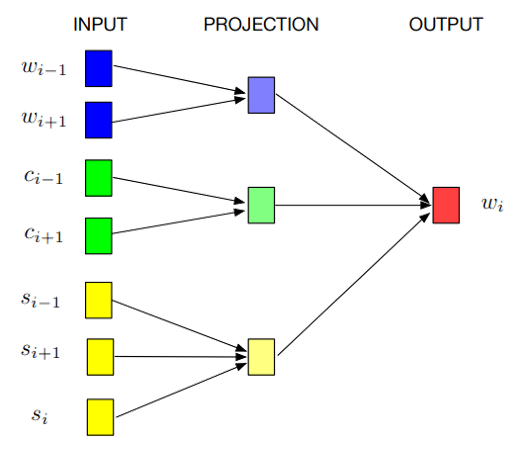
\includegraphics[scale=0.7]{../images/jwe_illustration.png}
	\caption{An illustration of JWE model proposed in \cite{yu2017joint}}
	\label{fig:jwe}
\end{figure}

As shown in the Figure \ref{fig:jwe} above, The JWE model is trained to predicts the present word from the context words in the same way as CBOW. The symbol $w$ represents words, $w_i$ is the current word, $w_{i-1}$ and $w_{i+1}$ are the context words. The symbol $c$ represents the characters of context words, $c_{i-1}$ is the characters of $w{i-1}$, and $c_{i+1}$ is the characters of $c_{i+1}$. The symbol $s$ represents the sub-characters of context words. $s_i$ is the sub-character components of $w_i$, and $s_{i-1}, s_{i+1}$ are the components of $w_{i-1}$ and $w_{i+1}$. For example, a word 智能 (intelligence) has two characters 智 (wisdom) and 能 (able), and each has sub-character components: 知, 日 and ㄙ, 月, 匕, 匕. The JWE model aims to maximize the sum of log-likelihoods of 3 conditional probabilities that come from the context words ($h_{i1}$), characters ($h_{i2}$), and sub-characters ($h_{i3}$).

\begin{equation}
L(w_i) = \sum_{k=1}^3\log P(w_i\mid h_{ik})    
\end{equation}

\subsubsection{cw2vec Model}

Inspired by fastText \cite{bojanowski2017enriching}, the authors of cw2vec \cite{cao2018cw2vec} proposed an n-gram feature based on the strokes of Chinese characters. They first split and transformed the text into stroke information, and mapped the strokes into 5 corresponding stroke ids, then merge the ids and generate n-gram features from these stroke ids. The diagram in the paper (Figure \ref{fig:cw2vec1}) shows the complete process.

\begin{figure}[h]
	\centering
	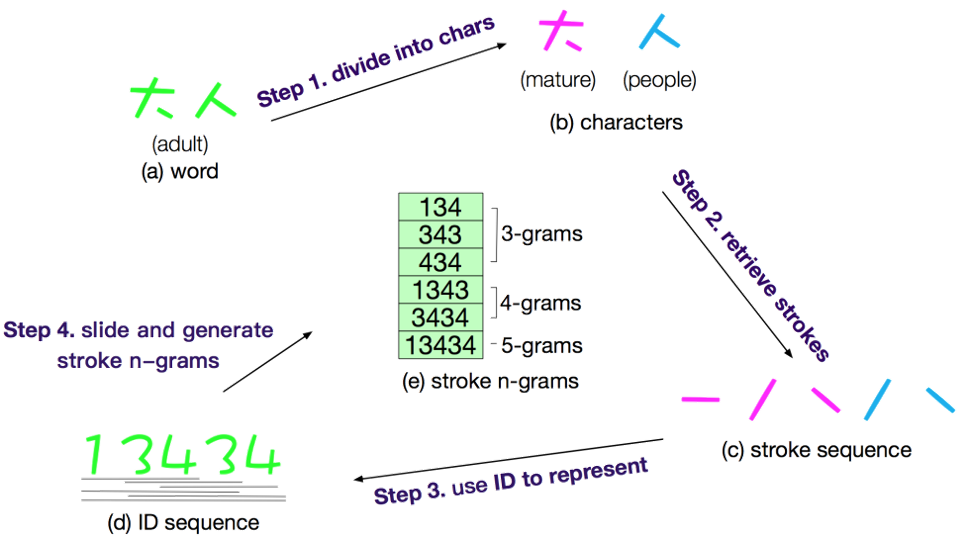
\includegraphics[scale=0.6]{../images/cw2vec_illustration1.png}
	\caption{The Process of generating stroke n-grams shown in \cite{cao2018cw2vec}}
	\label{fig:cw2vec1}
\end{figure}

The authors used Skip-Gram, a second method other than CBOW proposed by Word2Vec \cite{mikolov2013efficient}, as the base model, and replaced word inputs with stroke n-grams (Figure \ref{fig:cw2vec2}). It is mentioned in the paper that the final embeddings come from the contextual word vectors.

\begin{figure}[h]
	\centering
	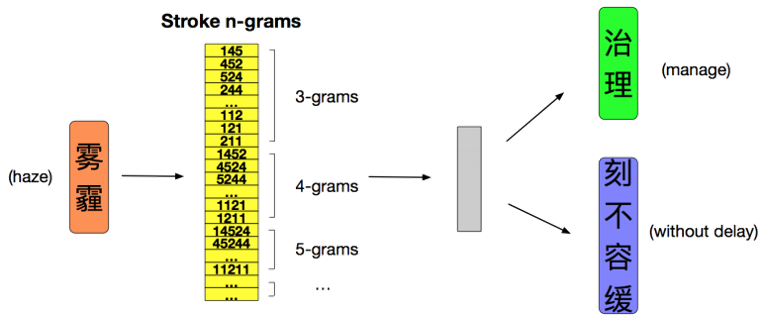
\includegraphics[scale=0.6]{../images/cw2vec_illustration2.png}
	\caption{An illustration of cw2vec model proposed in \cite{cao2018cw2vec}}
	\label{fig:cw2vec2}
\end{figure}

These word embeddings designed for Chinese all utilized the radicals or strokes in Chinese characters. No research in Chinese word embeddings has so far used phonetic information extracted from Chinese or Japanese as features.

\subsection{Phonetic Word Embedding} \label{sec:rw_pwe}

We will review studies that use phonetic information to construct word embeddings. These studies are closely related to our research, and we will learn from their practical differences and use them as the cornerstone for our experiments.

\subsubsection{Phonetic Encoding}

The study \cite{khan2019diversity} extracted sentences from Chinese or Western languages into phonetic encodings \footnote{The logogram encoding is also used as a feature but is not explained here. Random clustering is used for comparison purposes.}, which used \textit{Soundex}, \textit{NYSIIS}, \textit{Metaphone}, and \textit{Hanyu Pinyin} as the extraction algorithm. After that, they applied BPE \cite{sennrich_neural_2016} to tokenize the sentences and encodings, and trained separate embeddings from the sentences and each encoding (empty boxes in Figure \ref{fig:phonetic1}). Lastly, they concatenated the embeddings and fed them into the NMT system. 

\begin{figure}[h]
	\centering
	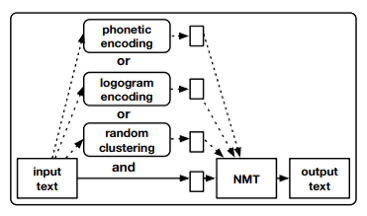
\includegraphics[scale=0.9]{../images/phonetic_encoding.png}
	\caption{Implementation of phonetic encoding proposed in \cite{khan2019diversity}}
	\label{fig:phonetic1}
\end{figure}

This paper did not explain the implementation of phonetic information in detail, but they had presented a hypothesis and verified it. That is, phonetics is a function that groups semantically distinct words. The words with the same pronunciation and spelling are usually distinguished by the different contexts.

\newpage

\subsubsection{Joint Textual and Phonetic Embedding}

This paper \cite{liu-etal-2019-robust} focused on using phonetic embedding to adjust the homophone noise problem, which is a frequent problem in a parallel corpus. For instance, when a single word in the source sentence is misplanted as a corresponding homophone (e.g., 有 (yǒu, to have) is wrongly replaced with 友 (yǒu, friend)), the model will read the wrong embedding and training in a wrong direction. The phonetic embedding can be seen as a feature to offset the errors that occur in semantic embeddings with homophone noise.

The paper trained the text (denoted by $a$) as semantic embedding (denoted by $\pi(a)$) and phonetic embedding (denoted by $\psi(a)$), and combined two embeddings with a configurable parameter (denoted by $\beta$) as follows:

\begin{equation}
	\pi([a, \psi(a)]) = (1-\beta) \times \pi(a) + \beta \times \pi(\psi(a)) 
\end{equation}

This study did not give the details of constructing embeddings, but they had mentioned that the best result occurs when the $\beta$ is $0.95$. That is, when they used 5\% of semantic embedding and 95\% of phonetic embedding, they obtained the best performance in their NMT system.

To summarize the findings in these related works. The phonetic encodings can emphasize the difference between semantically diverse sentences. The joint semantic-phonetic embedding also shows the robustness to noise in parallel corpora. All of these features can help improve the performance of the NMT system. However, the methods of using phonetic information as embeddings had been explored mainly in Chinese and Western languages. They also used \textit{Pinyin} instead of Bopomofo as the component to decompose Chinese characters. According to our study, no research has been proposed to apply and analyze phonetic information as an additional feature in Chinese and Japanese NMT systems.
